\documentclass{sig-alternate}
%%\documentclass[english]{hacked-sig-alternate}

\usepackage[usenames, dvipsnames]{color}
%\usepackage{times}
\usepackage{xspace}
\usepackage{textcomp}
\usepackage{wrapfig}
\usepackage{url}
\usepackage{amsmath, amssymb}
\usepackage[protrusion=true,expansion=true]{microtype}
%\usepackage{float}
\usepackage{alltt}
\usepackage{appendix}
%\usepackage{algorithm}
%\usepackage{algorithmicx}
%\usepackage{algpseudocode}
%\usepackage{texlive-science}
\usepackage{comment}
\usepackage{array,tabularx}
\usepackage{bussproofs}
%\usepackage{stmaryrd}

%\usepackage{txfonts}
\newcommand{\eat}[1]{}

\newtheorem{theorem}{Theorem}
\newtheorem{lemma}{Lemma}
\newtheorem{corollary}{Corollary}
%\theoremstyle{definition}
\newdef{example}{Example}
\newdef{definition}{Definition}

\newcommand{\naive}      {na\"{\i}ve\xspace}
\newcommand{\Naive}      {Na\"{\i}ve\xspace}

\newcommand{\jmh}[1]{{\textcolor{red}{#1 -- jmh}}}
\newcommand{\paa}[1]{{\textcolor{blue}{#1 -- paa}}}
\newcommand{\rcs}[1]{{\textcolor{green}{#1 -- rcs}}}
\newcommand{\nrc}[1]{{\textcolor{magenta}{#1 -- nrc}}}
\newcommand{\wrm}[1]{{\color{BurntOrange}{#1 -- wrm}}}

\begin{document}

%\conferenceinfo{ACM PODS}{'10 Indianapolis, IN, USA}
\title{Deterministic Concurrent Programming with Algebra}

\pdfinfo{/Title (Algebraic Programming for Parallel Asynchronous Systems)}

%%Format\titlenote{(Produces the permission block, copyright information and page numbering). For use with ACM\_PROC\_ARTICLE-SP.CLS V2.6SP. Supported by ACM.}}
%
% You need the command \numberofauthors to handle the "boxing"
% and alignment of the authors under the title, and to add
% a section for authors number 4 through n.

\numberofauthors{3}

\author{
\alignauthor William R.\ Marczak\\
\affaddr{UC Berkeley}\\
\email{wrm@cs.berkeley.edu}
\and
\alignauthor Neil Conway\\
\affaddr{UC Berkeley}\\
\email{nrc@cs.berkeley.edu}
\and
\alignauthor Joseph M. Hellerstein\\
\affaddr{UC Berkeley}\\
\email{hellerstein@cs.berkeley.edu}
}

\toappear{}

\maketitle

\begin{abstract}
Manipulating the ordering and batching of data for increased performance
of algorithms and systems is a time-honored tradition in computer science.
For instance, Codd's {\em order independence} underlies much of the
fields of query optimization and parallel databases, and is also implemented
in distributed systems such as MapReduce's {\em combiner} phase for partial merging.
The idea has a long tradition in algorithm design as well, for example in
deterministic {\em Las Vegas algorithms}, which employ randomness to break
the correlation between input instances and performance.  
These constructs and programming paradigms are widespread and helpful, but,
given a program, it is often hard to understand where reordering or introducing
disorder will preserve determinism.  Furthermore, the ordering aspect of
programs is too often a {\em cross-cutting concern}---changing the ordering
properties of a program involves changes to many modules or components.
We propose a programming language that decomposes algorithms
into ``algebra'' and ``ordering,'' in the vein of Kowalski's famous ``Algorithm
= Logic + Control'' formulation.  In our language, a programmer writes a
specification in ``algebra;'' the program's performance characteristics can
then be tuned without affecting its meaning by changing only the ``ordering.''
Our language
fosters a design pattern where programmers are dissuaded from adding
unnecessary ordering to the ``algebra'' specification; they are induced
to proactively write order-independent code so that the
order may later be customized.  We present the notion of ``timelines'' as an
interface between ``algebra'' and ``ordering:'' the ``ordering'' can be any
arbitrary code that produces a ``timeline,'' whereas the ``algebra'' is
restricted to ensure that program outcomes are independent of the
``ordering.''  We formally prove this property of our language and
demonstrate its applicability by considering a variety of case studies.
\end{abstract}

\section{Introduction} 
\label{sec:intro} 
Although distributed programming has become an essential and commonplace task,
it remains very challenging for most developers to write correct distributed
programs. The inherent difficulties of distributed computing---concurrency,
asynchrony, and partial failure---are exacerbated by the scale at which modern
distributed systems operate.

% remind reviewers that it's a database problem. can remove if accepted! 
Much of the discussion about distributed programming today revolves around data
management systems, and the tradeoffs between transactions and loose
consistency. Programmers using distributed transactions are relieved of
consistency concerns but often face significant performance and operational
challenges~\cite{Birman2009}. By contrast, programmers who use loosely
consistent systems can expect more predictable and low-latency performance, but
must reason explicitly about program correctness over inconsistent distributed
state.

In recent years there has been increased interest in techniques to help
programmers achieve correct program behavior without requiring strongly
consistent storage. This idea has been explored in two different frameworks,
\emph{Convergent Objects} and \emph{Monotonic Logic}.

\vspace{0.5em}\noindent
\textbf{Convergent Objects}: In this approach, a programmer writes encapsulated
object classes whose public methods guarantee certain properties regarding
message reordering and/or retry. For example, Statebox is an open-source library
that merges conflicting updates to data items in a key-value store; the user of
the library need only register commutative, idempotent merge
functions~\cite{statebox}. This approach has roots in research in
databases~\cite{Farrag1989,Garcia-Molina1983,Helland2009} and
groupware~\cite{Ellis1989,Sun1998}.  Shapiro et al.\ recently proposed a model
for these approaches called \emph{Conflict-Free Replicated Data Types} (CRDTs),
which formalizes these ideas in an algebraic framework~\cite{Shapiro2011b}.

The main problem with the CRDT approach is that its guarantees of correctness
are limited to an individual replicated data value, not to application logic in
general. For example, consider a distributed algorithmic trading service that
uses a CRDT to represent a mutable set \texttt{Portfolio}. Suppose one server
$M$ reads a local version of the set containing an element \texttt{BNNA} and
constructs an expected portfolio value $v = f(\mbox{\texttt{Portfolio}})$
derived from that version. Concurrently, \texttt{BNNA} is removed from the local
version of \texttt{Portfolio} at another server $N$. The CRDT can ensure that
$M$ and $N$ will eventually agree that \texttt{BNNA} is absent from the set, but
the application state at $M$ and $N$ may remain inconsistent unless the value
$v$ at $M$ is updated to reflect the removal of \texttt{BNNA}. Although the CRDT
maintains its own invariants, the programmer still bears the burden of ensuring
the consistency semantics of the entire program.

\vspace{0.5em} \noindent
\textbf{Monotonic Logic}: In recent work, we observed that the database theory
literature on non-monotonic logic provides a promising starting point for
reasoning about distributed consistency. Intuitively, a \emph{monotonic} program
computes more information over time---it never ``retracts'' an earlier
conclusion in the face of new information. We proposed the CALM
theorem~\cite{Hellerstein2010}, which established that all monotonic programs
are eventually consistent~\cite{Ameloot2011,dedalus-pods12-tr}. Monotonicity of
a Datalog-style program is straightforward to determine conservatively from
syntax, so the CALM theorem provides the basis for a simple analysis technique
for verifying the consistency of distributed programs~\cite{Alvaro2011}. We
realized the CALM analysis as part of Bloom, a Datalog-based DSL for distributed
programming~\cite{bloom}.

The original formulation of Bloom and CALM only validated consistency for programs that compute sets of facts that grow over time (``set monotonicity''); that is, ``growth'' is defined according to set containment. As a practical matter, this is overly conservative: several common distributed programming idioms that are monotonic do not satisfy syntactic monotonicity tests for Datalog. In particular, threshold tests over monotonic aggregate values (e.g., ``$\mathrm{max}(S) > k$'') and upward-moving mutable counters are both considered to be non-monotonic by the original CALM analysis.  As a result, the initial Bloom prototype advises the programmer to guard those constructs with strong consistency methods like Paxos~\cite{Lamport1998} or Two-Phase Commit. 

\subsection{A Hybrid Approach}
% The strengths and weaknesses of these two approaches appear complementary. CRDTs provide synchronization-free consistent objects, but cannot guarantee whole-program consistency. Bloom's CALM analysis guarantees whole-program consistency but is unable to verify a number of natural coordination-free mechanisms.
In this paper, we extend our previous work to accommodate the ideas underlying CRDTs. Instead of only allowing growth according to the set containment
partial order, we allow any user-defined partial order to be used.  
We do this by providing \emph{join semi-lattices} as a programming construct.
We give a
formal definition of this construct below, but the intuition is that the programmer provides a commutative, idempotent merge function (``least upper bound'')
that takes two input values and produces an output value that is not smaller
than either of the input values (according to the user's partial order). This
generalizes Bloom (and traditional Datalog), which assumes a fixed merge
function (set union) and partial order (set containment).
% Relate user-defined merge functions to merge functions in other contexts?
% (e.g., key-value store, COPS, Piccolo)

% Explain how lattices generalize monotonic datalog
It is attractive to incorporate join semi-lattices into logic programming,  but doing so raises challenges in language design, consistency analysis and efficient execution.  In this paper, we make the following contributions:
\begin{enumerate}
% \item
%   We present \baselang, a variant of Datalog that is defined over lattices. We
%   define a model-theoretic semantics for \baselang, and show that \baselang
%   generalizes Datalog.

\item
  We introduce \lang, an extension of Bloom that supports lattices. We detail
  the builtin lattice types provided by \lang and show how developers can
  define new lattices.
  
\item 
  We provide interfaces for consistency-preserving mappings across lattices via
  \emph{morphisms} and \emph{monotonic functions}.  This is critical for \lang
  and forms a useful extension to the CRDT framework as well.

\item 
  We generalize the CALM analysis to programs that contain both lattices and
  set-oriented collections, and show how lattices can be used to prove the
  confluence of several common distributed design patterns that were regarded as
  non-monotonic in Bloom. % XXX: revisit this

\item
  For efficient execution, we show how to extend the standard Datalog semi-naive
  evaluation scheme~\cite{Balbin1987} to support both lattices and traditional
  database relations. We also describe how an existing Datalog engine can be
  extended to support lattices with relatively minor changes.

\item
  Finally, we demonstrate the usefulness of lattices with two case studies.
  First we revisit the simple e-commerce scenario presented in Alvaro et al., in
  which clients interact with a replicated shopping cart
  service~\cite{Alvaro2011}. We show how \lang can be used to make the
  ``checkout'' operation monotonic, despite the fact that it requires
  aggregating over a distributed data set.

  Second, we use \lang to implement vector clocks and causal delivery, two
  standard building blocks for distributed programming. We show how both
  algorithms can be realized as monotonic \lang programs that are concise and
  readable.
\end{enumerate}

\section{Background}
\label{sec:background}

% XXX: should this be a distributed example?
\begin{figure}[t]
\begin{scriptsize}
\begin{lstlisting}
class ShortestPaths
  include Bud

  state do
    table :link, [:from, :to] => [:cost] (*\label{line:spaths-ddl}*)
    scratch :path, [:from, :to, :next_hop, :cost]
    scratch :min_cost, [:from, :to] => [:cost]
  end

  bloom do
    path <= link {|l| [l.from, l.to, l.to, l.cost]} (*\label{line:spaths-proj}*)
    path <= (link*path).pairs(:to => :from) do |l,p| (*\label{line:spaths-join-start}*)
      [l.from, p.to, l.to, l.cost + p.cost]
    end (*\label{line:spaths-join-end}*)

    min_cost <= path.group([:from, :to], min(:cost)) (*\label{line:spaths-group}*)
  end
end
\end{lstlisting}
\end{scriptsize}
\caption{All-pairs shortest paths in Bloom.}
\label{fig:bloom-spaths}
\end{figure}

In this section, we review the Bloom programming language and the CALM program
analysis.  We highlight a simple distributed program for which the CALM analysis
yields unsatisfactory results.

\subsection{Bloom}
\label{sec:bg-bloom}

Bloom is a Datalog-based domain-specific language (DSL) for distributed
programming~\cite{Alvaro2011,bloom}. The state of a Bloom program is represented
using \emph{collections} and computation is expressed as a bundle of declarative
\emph{statements}.  An instance of a Bloom program performs computation by
evaluating its statements over the contents of its local database. Bloom
instances communicate via asynchronous messaging, as described further below.

An instance of a Bloom program proceeds through a series of \emph{timesteps},
each containing three phases.\footnote{There is a precise declarative semantics
  for Bloom~\cite{dedalus}, but we describe the language operationally for the
  sake of exposition.} In the first phase, inbound events (e.g., network
messages) are received and represented as facts in collections. In the second
phase, the program's statements are evaluated over local state to compute all
the additional facts that can be derived from the current collection
contents. In some cases (described below), a derived fact is intended to achieve
a ``side effect,'' such as modifying local state or sending a network message.
These effects are deferred during the second phase of the timestep; the third
phase is devoted to carrying them out.

The initial implementation of Bloom, called \emph{Bud}, allows Bloom logic to be
embedded inside a Ruby program. Figure~\ref{fig:bloom-spaths} shows a Bloom
program represented as an annotated Ruby class. A small amount of imperative
Ruby code is needed to instantiate the Bloom program and begin executing it;
more details are available on the Bloom language website~\cite{bloom}.

\subsubsection{Data model}
\begin{table}[t]
\begin{tabular}{|l|p{2.32in}|}
\hline
\textbf{Name} & \textbf{Behavior }\\
\hline
\texttt{table} & Persistent storage.\\
\texttt{scratch} & Transient storage.\\
\texttt{channel} & Asynchronous communication. A fact derived into a \texttt{channel} appears in the
database of a remote Bloom instance at a non-deterministic future time.\\
\texttt{periodic} & Interface to the system clock.\\
\texttt{interface} & Interface point between software modules.\\
\hline
\end{tabular}
\caption{Bloom collection types.}
\label{tbl:bloom-collections}
\end{table}

The Bloom data model is based on \emph{collections}.  A collection is an
unordered set of \emph{facts}, akin to a relation in Datalog. The Bud prototype
adopts the Ruby type system rather than inventing its own; hence, a fact in Bud
is just an array of Ruby objects. Each collection has a \emph{schema}, which
declares the structure (column names) of the facts in the collection. A subset
of the columns in a collection form its \emph{key}: as in the relational model,
the key columns functionally determine the remaining columns. The collections
used by a Bloom program are declared in a \texttt{state} block. For example,
line~\ref{line:spaths-ddl} of Figure~\ref{fig:bloom-spaths} declares a
collection named \texttt{link} with three columns, two of which form the
collection's key. Ruby is a dynamically typed language, so keys and values in
Bud can hold arbitrary Ruby objects.

Bloom provides five collection types to represent different kinds of state
(Table~\ref{tbl:bloom-collections}). A \texttt{table} stores persistent data: if
a fact appears in a table, it remains in the table in future timesteps (unless it
is explicitly removed). A \texttt{scratch} contains transient data---the content
of scratch collections is emptied at the start of each timestep. Scratches are
akin to SQL views: they are often useful as a way to name intermediate results
or as a ``macro'' construct to enable code reuse. The \texttt{channel}
collection type enables communication between Bloom instances. The schema of a
channel has a distinguished \emph{location specifier} column (prefixed with
``\texttt{@}''); when a fact is derived for a channel collection, it appears in
the database of the Bloom instance at the address given by the location
specifier. The \texttt{periodic} and \texttt{interface} collection types do not
arise in our discussion in this paper; the interested reader is referred to the
Bloom website~\cite{bloom}.

\subsubsection{Statements}
\begin{table}
\begin{tabular}{|c|l|p{1.85in}|}
\hline
\textbf{Op} & \textbf{Name} & \textbf{Meaning} \\
\hline
\verb|<=| & \emph{merge} & lhs includes the content of rhs in the
current timestep \\
\hline
\verb|<+| & \emph{deferred merge} & lhs will include the content of rhs in the
next timestep \\
\hline
\verb|<-| & \emph{deferred delete} & lhs will not include the content of rhs
in the next timestep \\
\hline
\verb|<~| & \emph{async merge} & (remote) lhs will include the content of the
rhs at some non-deterministic future timestep\\
\hline
\end{tabular}
\caption{Bloom operators.}
\label{tbl:bloom-ops}
\end{table}

Each Bloom statement has one or more input collections and a single output
collection.  A statement takes the form: \\ \noindent
\mbox{\hspace{0.25in}\emph{$<$collection-identifier$>$ $<$op$>$
    $<$collection-expression$>$}}\\ \noindent
The left-hand side (lhs) is the name of the output collection and the right-hand
side (rhs) is an expression that produces a collection.  A statement defines how
the contents of the input collections should be transformed before being
included (via set union) in the output collection. Bloom allows the usual
relational operators to be used on the rhs (selection, projection, join,
grouping, aggregation, and negation), although it adopts a syntax intended to be
more familiar to imperative programmers. In Figure~\ref{fig:bloom-spaths},
line~\ref{line:spaths-proj} demonstrates projection,
lines~\ref{line:spaths-join-start}--\ref{line:spaths-join-end} perform a join
between \texttt{link} and \texttt{path} using the join predicate
\verb+link.to = path.from+ followed by a projection to four attributes, and
line~\ref{line:spaths-group} demonstrates grouping and aggregation. Bloom
statements appear in one or more \texttt{bloom} blocks. A Bloom program can also
include a \texttt{bootstrap} block, which contains statements that are evaluated
only once when a Bloom instance starts executing. \texttt{bootstrap} blocks are
typically used for initialization or configuration data.

Bloom provides several operators that determine \emph{when} the rhs will be
merged into the lhs (Table~\ref{tbl:bloom-ops}). The \verb|<=| operator performs
standard logical deduction: that is, the lhs and rhs are true at the same
timestep. The \verb|<+| and \verb|<-| operators indicate that facts will be
added or removed, respectively, from the lhs collection at the beginning of the
\emph{next} timestep. The \verb+<~+ operator specifies that the rhs will be merged into
the lhs collection at some non-deterministic future time. The lhs of a statement
that uses \verb+<~+ must be a channel; the \verb+<~+ operator captures
asynchronous messaging.

% XXX: does this need to be said?
Bloom allows recursion---i.e., the rhs of a statement can reference the lhs
collection, either directly or indirectly. As in Datalog, certain constraints
must be adopted to ensure that programs with recursive statements have a
sensible interpretation. For deductive statements (\verb+<=+ operator), we
require that programs be \emph{syntactically stratified}~\cite{Apt1988}: cycles
through negation or aggregation are not allowed (unless they contain a deferred
or asynchronous operator)~\cite{dedalus}.

\subsection{CALM analysis}
\label{sec:bg-calm}

Work on deductive databases has long drawn a distinction between
\emph{monotonic} and \emph{non-monotonic} logic programs. Intuitively, a
monotonic program only computes more information over time---it will never
``retract'' a previous conclusion in the face of new evidence.  In Bloom (and
Datalog), a simple conservative test for monotonicity is based on program
syntax: selection, projection, and join are monotonic, while aggregation and
negation are not.

The CALM theorem connects the theory of monotonic logic with the practical
problem of distributed consistency~\cite{Alvaro2011,Hellerstein2010}.  All
monotonic programs are ``eventually consistent'' or \emph{confluent}: for any
given input, all program executions result in the same final state regardless of
network non-determinism~\cite{Ameloot2011,dedalus-confluence}.  Hence, monotonic
logic is a useful building block for loosely consistent distributed programming.

According to the CALM theorem, distributed inconsistency may only occur at
\emph{points of order}: program locations where the output of an asynchronously
derived value is consumed by a non-monotonic operator.  This is because
asynchronous messaging results in non-deterministic arrival order, and
non-monotonic operators may be produce different conclusions when evaluated over
different subsets of their inputs.  For example, consider a Bloom program in
which collections $A$ and $B$ are fed by asynchronous channels and the program
sends a message whenever an element of $A$ arrives that is not in $B$. This
program is non-monotonic and exhibits non-confluent behavior: the messages sent
by the program will depend on the order in which the elements of $A$ and $B$
arrive.

We have implemented a conservative static program analysis in Bloom that follows
directly from the CALM theorem.  Programs that are free from non-monotonic
constructs are ``blessed'' as confluent: producing the same output on different
runs or converging to the same state on multiple distributed replicas.
Otherwise, programs are flagged as potentially inconsistent.  To achieve
consistency, the programmer either needs to rewrite their program to avoid the
use of non-monotonicity or introduce a coordination protocol to ensure that a
consistent ordering is agreed upon. Coordination protocols incur additional
latency and reduce availability in the event of network partitions, so in this
paper we focus on coordination-free designs---that is, monotonic programs.

\subsubsection{Limitations of set monotonicity}
The original formulation of the CALM theorem considered only programs that
compute more facts over time---that is, programs whose output \emph{sets} grow
monotonically. Many distributed protocols make progress over time, but their
notion of ``progress'' is often difficult to represent as a growing set of
facts. For example, consider the Bloom program in
Figure~\ref{fig:bloom-nm-quorum}. This program receives votes from a client
program (not shown) via the \texttt{vote\_chn} channel. Once at least
\texttt{QUORUM\_SIZE} votes have been received, a message is sent to a remote
node to indicate that quorum has been reached
(line~\ref{line:bloom-quorum-msg}). This program resembles a ``quorum vote''
subroutine that might be used by an implementation of Paxos~\cite{Lamport1998}
or quorum replication~\cite{Gifford1979}.

It is easy to see that this program makes progress in a semantically monotonic
fashion: the set of received votes grows and the size of the \texttt{votes}
collection can only increase, so once a quorum has been reached it will never be
retracted. Unfortunately, the current CALM analysis would regard this program as
non-monotonic because it contains aggregation (the grouping operation on
line~\ref{line:bloom-nm-quorum}).

To solve this problem, we need to introduce a notion of program values that
``grow'' according to a partial order other than set containment. We do this by
extending Bloom to operate over arbitrary lattices, rather than just the
set lattice.

%  We present a
% complete language in the following section, but the intuition can be observed in
% Figure~\ref{fig:lattice-quorum}. Votes are accumulated into a set lattice
% (line~\ref{line:quorum-set-accum}), but the size of the set is represented as an
% \texttt{lmax} lattice (line~\ref{line:quorum-lmax}): that is, a number that
% never decreases. Hence, a threshold test ``$\ge k$'' on an \texttt{lmax} lattice
% is monotonic map onto the boolean lattice: that is, the \texttt{quorum\_done}
% predicate goes from false to true (and then remains true).

\begin{figure}[t]
\begin{scriptsize}
\begin{lstlisting}
QUORUM_SIZE = 5
RESULT_ADDR = "example.org"

class QuorumVote
  include Bud

  state do
    channel :vote_chn, [:@addr, :voter_id]
    channel :result_chn, [:@addr]
    table   :votes, [:voter_id]
    scratch :cnt, [] => [:cnt]
  end

  bloom do
    votes      <= vote_chn {|v| [v.voter_id]}
    cnt        <= votes.group(nil, count(:voter_id)) (*\label{line:bloom-nm-quorum}*)
    result_chn <~ cnt {|c| [RESULT_ADDR] if c >= QUORUM_SIZE} (*\label{line:bloom-quorum-msg}*)
  end
end
\end{lstlisting}
\end{scriptsize}
\caption{A non-monotonic Bloom program that waits for a quorum of votes to be received.}
\label{fig:bloom-nm-quorum}
\end{figure}

\section{Case Study}
\label{sec:case}

%%\wrm{Re-do case studies in Bud} \wrm{Break cart development down into
%%iterations} \wrm{How does the language naturally lead us to an order
%%independent style?  Talk about inserting all sorts of exotic stuff like queues
%%if we want a highly order-dependent imperative style.}

\begin{comment}

\jmh{We discussed the following on the phone.  (1) Handle shopping in two styles: destructive updates, and disorderly accumulation of increment/decrement.  (2) Do analysis on them to detect need for coordination in only the first, show that (annotated) 2PC removes the compiler warning.  (3) Deploy destructive+2PC on EC2 and show practical benefits of avoiding coordination.  (4) Evolve the program with new rules for checkout and/or inventory, show how the disorderly version is no longer monotonic.  Fix that  with 2PC where needed.  Also make sure the destructive version works with the new rules.  Now show that the disorderly version is still better than the destructive one, by coordinating only where needed.}

\jmh{Finally, show what would happen if you didn't coordinate the inventory bit, but tracked taint.  Note that tainted output is the stuff where programmers need to write compensation logic.}

\end{comment}

%%In this section, we implement two different styles of distributed shopping cart
%%applications in Bud.  First, we implement a ``destructive,'' overwriting
%%shopping cart application using a simple key-value store implemented in Bud.
%%Second, we implement a ``disorderly'' cart which accumulates updates in a 
%%set-wise fashion and describes how to combine the updates into a final result.

\jmh{Blah blah intro.}

We begin with a shopping
cart built on a key-value store abstraction.  Each cart is a pair \texttt{[key,value]}, where \texttt{key} is a unique 
session identifier, and \texttt{value} is a Ruby array
representing the set of items contained in the cart at any time.  Addition
and deletion actions to a cart result in ``destructive'' overwrites,
replacing the value associated with the key with a new array reflecting
the additions.  Deletion from an empty cart is ignored. 

Figure~\ref{fig:pdg-destructive} shows the Bloom code for this design.
The 
\textbf{scratch} \texttt{kvstore} is defined by the KeyValueStore module (XXX lines of Bloom not shown here), 
which the shopping cart extends via inheritance.
%; it is used in a manner analogous to the \emph{put} function for hash tables.  
The set of shopping carts, represented by the persistent \textbf{table} \texttt{bigtable}, is kept 
consistent across replicas by shipping \texttt{kvstore} tuples to other servers.
%%\jmh{Line numbers seem messed up.}

We begin describing the logic from the outside:
cart updates are transmitted from the client in line 28,
thereafter appearing in the \texttt{action\_msg} \textbf{channel} at a server replica.
\jmh{which server replica?  all server replicas??}
For each such arriving tuple,
line 2 probes the \texttt{bigtable} collection for a matching
session.  If none is found (i.e., the cart did not previously exist), lines 2-6 are evaluated, generating
the key with an appropriately initialized array. 
Otherwise the join conditions
in lines 10-11 will be met and lines 12-18 will instead be evaluated, ``replacing'' the value at the next timestep with an appropriately-modified new value.
Finally, when a checkout message is received, the value in \texttt{bigtable}
associated with the given session is extracted (via the join on lines 22-23)
and sent back to the client.

Figure~\ref{fig:} shows an alternative shopping cart implementation, in which
updates are accumulated in a disorderly fashion and summarized only at 
checkout.  Line 0 appends all client updates to the persistent table 
\texttt{cart\_action}.  Lines 2-3 define \texttt{action\_cnt} as an aggregate
over \texttt{cart\_action}, in the style of an SQL group-by statement: for
each item associated with a cart, we separately count the number of times it was added and the number of times it was deleted.
\jmh{what's up with lines 5-9?  initialize number of deletions to 0...to avoid failed join of additions with no deletions, right?  Maybe less confusing to do another rule for status that antijoins additions to deletions.  Or we could hack up an outerjoin syntax.}
\paa{I've frequently wanted an outerjoin syntax.  anti join? do you mean a 
'subquery' with unlesss..include? ?}
Lines 11-16 define the collection \texttt{status} as a 3-way
join between the \texttt{checkout} message and two copies of 
\texttt{action\_cnt} (one corresponding to additions and one to deletions),
and for each item, compute its final quantity in the cart as the difference of the two counts
in line 14.  A \texttt{response} message containing the quantity is then sent 
to the client in lines 18-22.  Because the disorderly implementation does not
use a separate storage system, it must replicate its own state to replicas 
via multicast (lines 24-26).


\begin{figure}[t]
\begin{scriptsize}
\begin{verbatim}

0: kvstore <= action_msg.map do |a|
1:   if not bigtable.map{|b| b.key}.include? a.session
2:     if a.action == "Add"
3:       [a.server, a.client, a.session, a.reqid, [a.item]]
4:     elsif a.action == "Del"
5:       [a.server, a.client, a.session, a.reqid, []]
6:     end
7:   end
8: end
9: 
10: kvstore <= join([bigtable, action_msg]).map do |b, a|
11:   if b.key == a.session
12:     if a.action == "Add"
13:       [a.server, a.client, a.session, a.reqid, b.value.push(a.item)]
14:     elsif a.action == "Del"
15:       copy = b.value.clone;
16:       copy.delete_at(copy.index(a.item));
17:       [a.server, a.client, a.session, a.reqid, copy]
18:     end
19:   end
20: end
21:
22: response_msg <+ join([bigtable, checkout_msg]).map do |s, c|
23:   if s.key == c.session
24:     [c.client, c.server, s.key, s.value]
25:   end
26: end
27: 
28: action_msg <+ client_action.map{|a| a}


\end{verbatim}
\end{scriptsize}
\caption{Destructive Cart Implementation}
\label{fig:pdg-destructive}
\end{figure}

\begin{figure}[t]
\centering
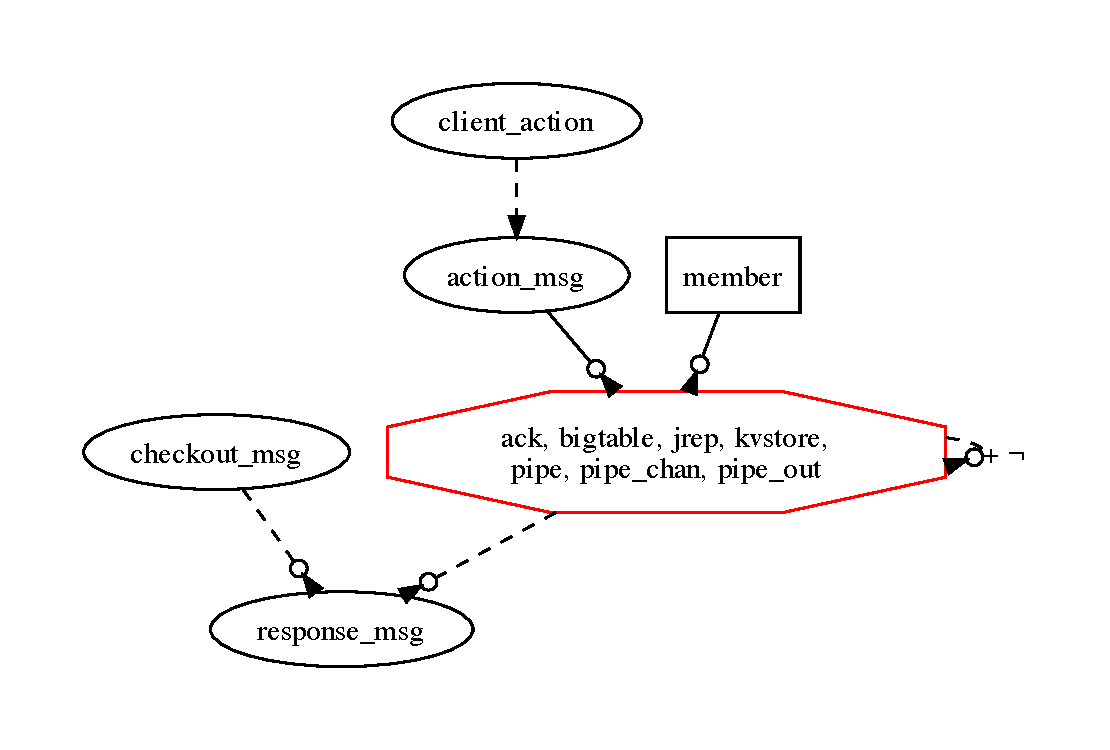
\includegraphics[width=0.9\linewidth]{fig/destructive.pdf}

\caption{Destructive Cart Analysis, with temporal cycles collapsed}
\label{fig:pdg-destructive-analysis}
\end{figure}


\subsection{Analysis}


For each cart, we apply whole-program analysis techniques to discover points of 
order.  The Bud interpreter automatically generates
a graphical representation of the dependency graph of collections through rules,
(and hence the 
flow of tuples) as a staged dataflow.  Each node in the graph is either
a collection or a cluster of collections (as described below).  A directed edge from node $A$ to node $B$ captures the fact that $B$ is in the lhs of a Bloom statement with $R$ in the rhs (or in a join expression in the rhs).  Edges are annotated based on the operators and lhs types in the rules.  Rules that involve synchronous timesteps---i.e. a \texttt{$<$+} operator with a {\bf table} lhs---are marked with a $+$.  Rules that involve asynchronous messaging---i.e., a \texttt{$<+$} operators with a {\bf channel lhs}---are indicated by a dashed line.  Nonmonotonic rhs predicates result in edges marked with a $\lnot$.  Strongly connected components having both a $\lnot$ and a $+$ edge are grouped into ``temporal clusters'', 
%%\jmh{capturing what? the fact that they must recurse over multiple timesteps?}
collapsing the mutually dependent collections into a single node.  All edges
incident to a temporal cluster, including the self-edge, are points of order,
as are any negated edges.
%%Individual monotonic components 
%%(or strata) are surrounded by a dotted rectangle.  A point of order occurs
%%wherever an edge crosses strata, or at any self-edge attached to a temporal cluster.
Points of order are indicated by lightning bolts.

To resolve a point of order, the programmer may add coordination logic, which typically ensures  ordered delivered tuples, and/or guarantees that a boundary condition has been irrevocably crossed (e.g., there will be no more tuples).
% Instead of reanalyzing the augmented program, we associate coordination code
% with an annotation that can
% be interpreted as a contract about a point of order.  Such contracts will
% typically guarantee an ordering over arriving tuples, or guarantee a 
% a barrier-passing condition (e.g., indicating that there will be no more tuples).

\jmh{the subsequent discussion should be pared down and made simple.  updates are non-monotonic.  we see it in the points of order.  If we resolve using coordination a la 2PC, we get a round of coord for every client action.  This is the kind of thing Amazon didn't like for availability.  However, if we examine the disorderly figure, we see that the point of order is at checkout only, which is what Amazon wanted.}
%%Intuitively, the ``destructive'' cart based on
%%array mutation should be non-monotonic due to the transience of its state; this should make it sensitive to the order
%%of its inputs.
Although there is no syntactically obvious non-monotonicity in the destructive
cart code as shown, the underlying key-value store uses the \texttt{$<$-} operator to model updateable state, which results in non-monotonicity.\footnote{Our full-length paper expands the SCC to analyze the
key-value store in detail.}
The global analysis shown in Figure~\ref{fig:pdf-destructive}
indicates that there are
points of order between \texttt{action\_msg} and the temporal cluster,
and between the temporal cluster and itself.
%%This means that the arrival 
%%timing and ordering of both client updates (via \texttt{iaction}) and
%%server replication (via the meta-edge in the temporal cycle from 
%%\texttt{kvstore} to itself) may affect the
%%end results.  
To ensure a consistent final state across all replicas, we may require coordination
between client and server at every update to the cart, and between the 
server and all replicas at each update.   

%%We can easily achieve coordination without modifying the cart implementation
%%by redefining the key-value store to extend
%%a reliable or quorum-based delivery module instead of the best-effort module
%%that the basic key-value store extends, and require acknowledgement from a server or a %%quorum of servers, respectively.
%%The simplest (and least performant) approach is to require unanimous quorum,
%%approximating ``eager replication''~\cite{dangers} via two-phase commit.
A programmer could resolve this point of order by adapting the key-value store
to require reliable delivery to all replicas before acknowledging a client update, by
making the key-value store inherit from a superclass providing a reliable delivery
abstraction (6 LOC).
Such ``eager replication''~\cite{dangers} would incur a cost of a round of messages
per server per client update, and substantially decrease system throughput.  
Because we only care about the set of elements contained in the value array
and not its order, we might be tempted to argue that 
the shopping cart application is eventually consistent
when asynchronously updated, and forego the synchronization.  Unfortunately, such informal reasoning can hide serious bugs: consider what happens if a delete update is received
before the addition it was intended to cancel.



\begin{figure}[t]
\begin{scriptsize}
\begin{verbatim}
0:  cart_action <= action_msg.map { |c| [c.session, c.item, c.action, c.reqid] }
1:
2:  action_cnt <= cart_action.group([cart_action.session, 
3:    cart_action.item, cart_action.action], count(cart_action.reqid))
4:
5:  action_cnt <= cart_action.map do |a| 
6:    unless cart_action.map{|c| [c.session, c.item] if c.action == "D"}.include? [a.session, a.item] 
7:      [a.session, a.item, 'D', 0]
8:    end 
9:  end
10: 
11: status <= join([action_cnt, action_cnt, checkout]).map do |a1, a2, c| 
12:   if a1.session == a2.session and a1.item == a2.item 
13:   and a1.session == c.session and a1.action == "A" and a2.action == "D"
14:     [a1.session, a1.item, a1.cnt - a2.cnt] if (a1.cnt - a2.cnt) > 0
15:   end
16: end
17:
18: response_msg <= join([status, checkout]).map do |s, c| 
19:   if s.session == c.session
20:     [c.client, c.server, s.session, s.item, s.cnt]
21:   end
22: end
23: 
24: action_msg <+ join([action_msg, member]).map do |a, m|
25:   [m.player, a.server, a.session, a.item, a.action, a.reqid]
26: end
27: 
28: checkout_msg <+ join([checkout_msg, member}).map do |c, m|
29:   [m.player, c.server, c.session, c.reqid]
30: end


\end{verbatim}
\end{scriptsize}
\caption{Disorderly Cart Implementation}
\label{fig:pdg-disorderly}
\end{figure}

\begin{figure}[t]
\centering
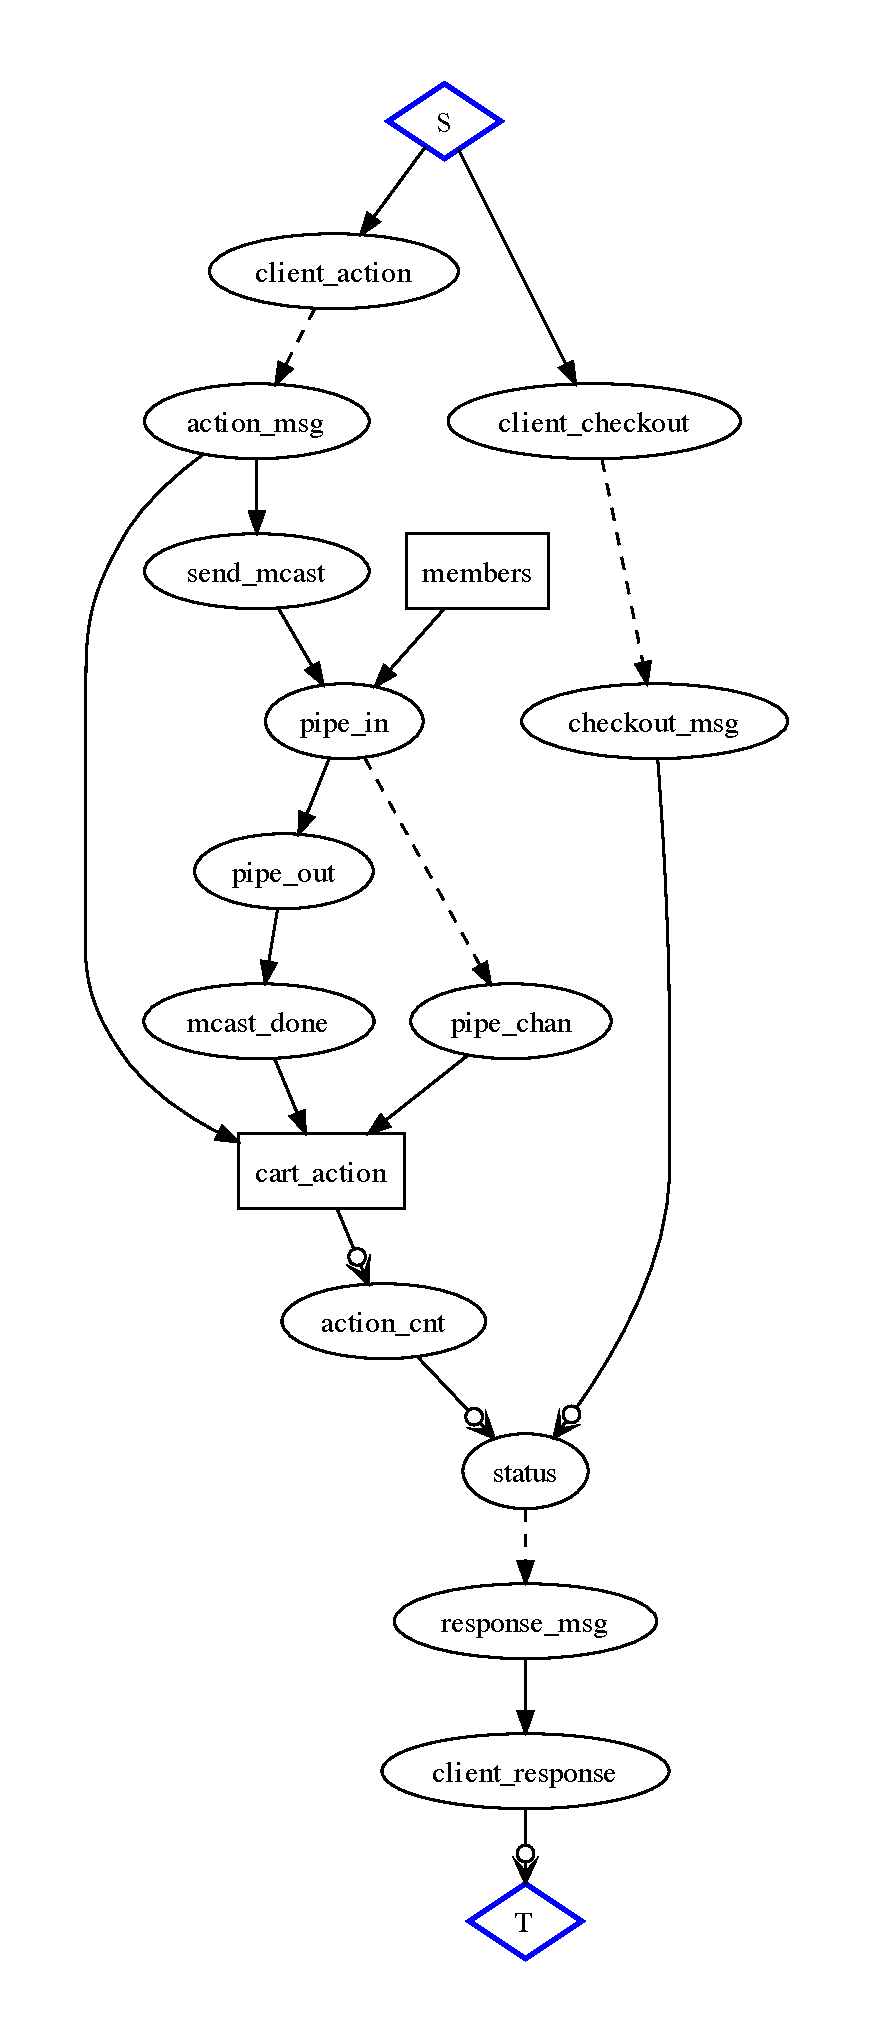
\includegraphics[width=0.7\linewidth]{fig/disorderly.pdf}
\caption{Disorderly Cart Analysis}
\label{fig:pdg-disorderly-analysis}
\end{figure}




Turning our attention to the disorderly figure,
\begin{comment}
 shows dotted lines indicating that 
\texttt{action\_msg} (owned by the server) is derived from \texttt{client\_action} 
(owned by the client) via an asynchronous message, and that \texttt{action\_msg} 
derives itself via messages when it is replicated.  However, the analysis
shows that because these derivations are strictly monotonic, no points of
order are crossed.  Hence, clients may send and servers may replicate 
updates without any coordination: regardless of timing and ordering, the end
result will be the same.

The analysis does indicate a point of order at checkout, when a \texttt{checkout}
message is joined with an aggregate over the set of updates.  While the 
accumulation of state has been monotonic, summarization of the cart state
requires us to assume (or prove) that there will be no further updates.
Consider a checkout message and a final update message racing from a client
to one of the replicas: the order in which they arrive will surely affect
the contents of the response message.  
\end{comment}
we see that communication (via \texttt{action\_msg}) between client and server
and between servers and replicas crosses no points of order, so all such
communication will converge to the same final state without coordination.
There is, however, a point of order at checkout, when a \texttt{checkout}
message is joined with an aggregate over the set of updates.  While the 
accumulation of state has been monotonic, summarization of the cart state
requires us to assume (or prove) that there will be no further updates.
Consider a checkout message and a final update message racing from a client
to one of the replicas: the order in which they arrive will surely affect
the contents of the response message.  
We need only coordinate once per session to
ensure that the response to the client is deterministic.

Like embarrassing parallelism in parallel computing, strictly monotonic programs
are rare in the distributed systems domain.  In this running example we studied
two candidate implementations of a simple distributed application with the aid of
our tool, and discovered that both have points of order.  Deciding that the disorderly
approach is ``better'' required us to apply domain knowledge: checkout happens
once per session, and is a more efficient coordination point than state update and replication, 
which occur repeatedly -- this is not unlike synchronizing on read rather than write 
in write-dominant systems generally.  Our analysis assisted us by highlighting the few locations where program correctness may depend upon costly synchronization, which may
result in decreased throughput and availability.  

\jmh{Challenge text that was kicking around and needs to be addressed here: we don't really say how we discourage a programmer from a destructive implementation, or help them migrate from that implementation to a better one.  Ideally we'd find ways to ``push back'' coordination requirements to local nodes and/or points of the program that don't have latency constraints.}


\section{Related Work}
\label{sec:relwork}
The shopping cart case study in Section~\ref{sec:case} was motivated by the
Amazon Dynamo paper~\cite{dynamo}, as well as the related discussion by Helland
and Campbell~\cite{quicksand}. Systems with loose consistency requirements have
been explored in depth by both the systems and database management communities
(e.g.,~\cite{sagas,leases,dangers,bayou}); we do not attempt to provide
an exhaustive survey here.

The Bloom language is inspired by earlier work that attempts to integrate
databases and programming languages.  This includes early research such as
Gem~\cite{gem} and more recent object-relational mapping layers like Ruby on
Rails.  Unlike these efforts, Bloom is targeted at the development of both
distributed infrastructure and distributed applications, so it does not make any
assumptions about the presence of a database system ``underneath it.''  Given
our prototype implementation in Ruby, it is tempting to integrate Bud with
Rails; we have left this for future work.

Our work on Bloom bears a resemblance to the Reactor
language~\cite{reactors}. Both languages target distributed programming and are
grounded in Datalog. Moreover, both languages combine declarative rules and
state into a single program construct. While Bloom uses a syntax inspired by
object-oriented languages, Reactor takes a more explicitly agent-oriented
approach. Reactor also includes synchronous coupling between agents as a
primitive; we have opted to only include asynchronous communication as a
language primitive and to provide synchronous coordination between nodes as a
library. Another significant different is that, like many rule-based languages,
Reactor includes some imperative constructs (e.g., \ldots), whereas rules in
Bloom are purely declarative.

Another recent language related to our work is Coherence~\cite{coherence}, which
also embraces ``disorderly'' programming. Unlike Bloom, Coherence is not
designed for distributed computing and is not based on logic programming.

There is a long history of attempts to design programming languages more
suitable to parallel and distributed systems; for example, Argus~\cite{argus}
and Linda~\cite{linda}.  Again, we do not hope to survey that literature here.
More pragmatically, Erlang is an oft-cited choice for distributed programming in
recent years.  Erlang's features and design style encourage the use of
asynchronous lightweight ``actors.''  As mentioned previously, we did a simple
Bloom prototype DSL in Erlang (which we cannot help but call ``Bloomerlang''),
and there is a natural correspondence between Bloom-style distributed rules and
Erlang actors.  However there is no requirement for Erlang programs to be
written in the disorderly style of Bloom. It is not obvious that typical Erlang
programs are significantly more amenable to a useful points-of-order analysis
than programs written in any other functional language.  For example, ordered
lists are basic constructs in functional languages, and without program
annotation or deeper analysis than we need to do in Bloom, any code that
modifies lists would need be marked as a point of order, much like our
destructive shopping cart.  We believe that Bloom's ``disorderly by default''
style encourages more disorderly programming; we know that its roots in database
theory bore fruit in terms of our analysis.  While we would be happy to see the
analysis ``ported'' to currently popular distributed programming environments,
it may be that design patterns using Bloom-esque disorderly programming are the
natural way to achieve this.


\bibliographystyle{abbrv}
\bibliography{pods}

%\appendix
%\section{Proof of Lemma 1}
\begin{proof}
%First, we prove an isomorphism between stable models, and finite prefixes of stable models.  Scan a stable model of a program timestamp by timestamp.  
We first present an algorithm for computing ultimate models, and argue that the algorithm computes exactly the ultimate models of the \lang program.  We then argue this algorithm can be run on our operational formalism, and show how operational traces correspond with prefixes of stable models.

Any \lang program without asynchronous rules is a $\text{Datalog}_{1S}$ program, and the algorithm given in~\cite{tdd} computes its ultimate model in polynomial space\footnote{The class of {\em multi-seperable}~\cite{tdd-poly} \lang programs, which comprises all \lang programs $P$ with guarded asynchrony and persisted EDB, and their coordinations $\textsc{Coord}(P)$, can be executed in polynomial time in the size of the input.} in the size of the input.  The algorithm evalutes the program for $2^G + e$ consecutive timesteps, where $G$ is the number of instantiations of the non-temporal attributes of the program rules using all combinations of constants in the Herbrand Universe, and $e$ is the maximum timestamp of any EDB fact.  At each step, the algorithm updates information on observed periodicities of facts.  When the algorithm terminates, any fact with a periodicity of 1 is regarded as part of the ultimate model.

For asynchronous rules, the natural distributed analog of the above algorithm simultaneously executes one instance for each node \dedalus{n}, using values of $G$ and $e$ computed from $E_{\text{\dedalus{{\scriptsize n}}}}$.  Each instance has its own local clock, which corresponds to the timestamp attribute in the model-theoretic semantics.  Nodes communicate over channels with arbitrary delay and message re-ordering.  When a remote node \dedalus{m} derives a fact at \dedalus{n}, it encloses its local clock value, \dedalus{t}; \dedalus{n} must consider this fact at his local time \dedalus{t} or later, in the style of Lamport Clocks.  Note that this behavior is equivalent to the model-theoretic semantics of remote asynchronous rules: remote deductions are visible at the destination at a time later than the body temporal attribute at the source.  Further, note that Lamport Clocks only introduce the constraint that if message $a$ ``happens before'' $b$, in other words $a$ directly or transitively causes $b$ to be sent, then $T(a) < T(b)$.  If $a$ and $b$ are concurrent, there is some execution where $T(a) \geq T(b)$.

When \dedalus{n} processes a received message, the number of constants available to \dedalus{n} may increase, and thus the node's $G$ may increase to $G'$.  Furthermore, the node may need to execute over this new fact for $2^{G'}$ additional timesteps.  If only finitely many messages are sent, this algorithm terminates, and requires polynomial space.  In the case that infinitely many messages are sent, we only need to process each message $2^{G'}$ times: the maximum period of any fact is $2^{G'}$, as every incoming fact needs to have a chance (in some execution) to join with any deduction (with which it is ``concurrent'') at any time during its period.  Keeping track of the number of times we have seen each fact also requires polynomial space.  When the algorithm is done running for $2^{G'}$ steps, it pauses, waiting for new network input that it has not seen enough times.  If all nodes are paused and no outstanding messages exist, then the collection of all period 1 facts at all instances of the algorithm comprises an ultimate model.

We claim that the algorithm can generate every ultimate model---every message has the opportunity to join with another concurrent message or its transitive consequents at any point during their period, and has the opportunity to join with a causally related message during the range of times allowed by the model-theoretic constraint (identical to the Lamport Clock condition used in the algorithm).  Furthermore, the set of all facts, and their local timestamps, comprises a prefix of a stable model.

Note that we can execute this algorithm straightforwardly on our operational formalism.  Evaluating a single timestamp of a \lang program corresponds to the evaluation of a Datalog program, which is a polynomial time computation, and the Turing Machines can also maintain the necessary state about periods and message counts.
%2) Intuitively, the operational model is based on n Turing Machines, one per value of node(), which independently step sequentially through time and communicate via channels with
%non-deterministic delay.  At each timestep t they run a datalog fixpoint computation that evaluates P on ``projection(E_n, t)'' (notation needed); this takes polynomial
%time~\cite{immerman}.  At the end of this fixpoint there are three sets of relevant facts: local, synchronous facts that have timestep t+1 and become part of ``projection(E_n,
%t)'', local asynchronous facts whose timestep is chosen non-deterministically to be greater than t and become part of later timesteps, and remote asynchronous facts.  The
%timestamps in this third class of facts are chosen non-deterministically ``at the receiver'' to model delay, in a way that observes traditional causality
%restrictions~\cite{lamportclocks}.
%3) Any \lang program without  async rules is a Datalog_{1S} program, and the above intuition is captured by the algorithm given in~\cite{}, computing an ultimate model in
%polynomial space in the size of the input.  In the presence of asynchronous rules, this formalize needs to be expanded to account for the asynchronous advancement of time through
%\dedalus{successor} at each node.  The PSPACE guarantees of~\cite{} are not shown to hold for such programs, but in Appendix Foo we show that the following Lemma holds for all
%\lang programs under this model
\end{proof}

\section{Proof of Lemma 2}
\begin{proof}
We begin by assuming that \dedalus{node} contains the identifiers of each of the $n$ nodes.  Since the atemporal fragment of \lang is FO[LFP], we can represent a polynomial-time bounded Turing Machine using only atemporal rules in \lang~\cite{immerman-ptime}.  In addition to normal operations, the Turing Machine can place items into a queue---\cite{dedalus} shows how to model queues in \lang---or send messages to other nodes---modeled by an asynchronous communication rule with \dedalus{queue} in the head.  A node persists the contents of the tape across time if the queue is empty, using a rule like \dedalus{tape(\dbar{X})@next <- tape(\dbar{X}), !queue(\dbar{\_});}.  If the queue is non-empty, the computation skips a timestamp (leaving \dedalus{tape} empty), and then atomically copies the contents of \dedalus{queue} to \dedalus{tape}.  The ultimate model of this program is exactly the final contents of the tape on every node if the computation halts.  Otherwise, the program's ultimate model is empty: \dedalus{tape} facts only exist every other timestamp, and for any Turing Machine predicate \dedalus{r} we can create \dedalus{r'}, and create a mutual recursive cycle to ensure neither \dedalus{r} nor \dedalus{r'} contains facts at every timestamp:

\begin{Dedalus}
r(\dbar{X})@next <- r'(\dbar{X});
r'(\dbar{X})@next <- r(\dbar{X});
\end{Dedalus}

We can play a somewhat similar trick for \dedalus{queue} by having local messages alternate between going into \dedalus{queue} and \dedalus{queue'}.  Thus, no local queue message will be part of the ultimate model.  Remote messages will still go into \dedalus{queue}: this still leaves the case that the exact same message repeatedly arrives at a node at every timestamp forever, by chance.  We can dispense of this case by assuming the channels interconnecting the Turing Machines forbid it.
\end{proof}

\section{Proof of Lemma 3}
\begin{proof}
Our proof proceeds via construction of a two counter machine in \lang, inspired by the construction in~\cite{undecidable-datalog}.

We represent the state of a two counter machine using the \linebreak \dedalus{cnfg(T,S,C1,C2)} relation, where \dedalus{T} represents ``time'' (note this is not the same as the \lang temporal attribute), \dedalus{S} is the state, and \dedalus{C1} and \dedalus{C2} are the values of the two counters.  In order to support our two instructions, $inc$ and $dec$, we would like to make use of the \dedalus{successor} relation.  However, \lang conventions forbid the use of this infinite relation outside of the timestamp attribute.  Thus, we posit the \dedalus{fin\_succ(X,Y)} EDB relation, which is meant to represent a finite prefix of the \dedalus{successor} relation.  Since it is EDB, its contents may be arbitrary.  If \dedalus{fin\_succ} is malformed, then the machine's execution may be incorrect.  In particular, our model of the machine may accept an input, whereas the actual machine would not have accepted that input.  We illustrate how to constrain the contents of \dedalus{fin\_succ} below:

\begin{Dedalus}
malformed() <- fin_succ(_,0);
malformed() <- fin_succ(X,Y), fin_succ(X,Z), Y != Z;
malformed() <- fin_succ(Y,X), fin_succ(Z,X), Y != Z;
malformed() <- fin_succ(X,Y), X >= Y;
\end{Dedalus}

For a given EDB, the two counter machine either halts in the accepting state or halts in a non-accepting state.  It cannot run forever since the EDB (in particular, the \dedalus{fin\_succ} relation) is finite.

We construct a \lang program that nondeterministically decides to either run the machine on the input provided (and for the length of \dedalus{fin\_succ} provided, or declare that the machine will never accept without running it.  If the machine ever accepts some input, this induce two different ultimate models---one generated by a trace where we run the machine and it accepts, and one generated by a trace where we decide to not run the machine, and thus we implicitly reject.  We describe the program below. 

Initially, we nondeterministically decide whether to run the machine or not by sending two messages (0 and 1) to a remote node (\dedalus{decider}).  If both message arrive simultaneously, then the decider responds to run the machine.  Otherwise, the decider responds to declare failure:

%\jmh{should we use a hashmark for constants?  I would say no.}
\begin{Dedalus}
//send two messages to the decider
message(#D, 0)@async <- decider(D);
message(#D, 1)@async <- decider(D);

//decider responds to computer
run_machine(#computer)@async <- message(0),
                                message(1);
declare_failure(#computer)@async <- message(0),
                                    !message(1);
declare_failure(#computer)@async <- !message(0),
                                    message(1);
\end{Dedalus}

Each mapping in the transition function is expressed by a \lang rule with \dedalus{!malformed()} and \dedalus{!declare\_failure()} in its body.  For example, the rule $\delta(3, > =) = (7, inc, dec)$ would be represented as:

\begin{Dedalus}
cnfg(S,7,D1,D2) <- cnfg(T,3,C1,C2), C1 > 0, C2 == 0,
                   fin_suc(T, S), fin_succ(C1, D1),
                   fin_succ(D2, C2), !malformed(),
                   !declare_failure();
\end{Dedalus}

We declare success or failure as follows:

\begin{Dedalus}
reject() <- !accept();
accept() <- cnfg(20,_,_); //20 is the accepting state
accept()@next <- accept();
\end{Dedalus}

If we choose to declare failure, or the machine halts in a non-accepting state---whether it is due to incompleteness or malformedness of \dedalus{fin\_succ}, or actual halting---then the ultimate model will contain \dedalus{reject}.  If the machine halts in an accepting state, then the ultimate model will contain \dedalus{accept}.  Thus, if we can decide confluence of this program, then we can decide whether there is any input for which an arbitrary two-counter machine halts.
\end{proof}


%%\section{attic}

\subsection{Kinds of Relations}
    
%%\jmh{Ack ... deductive rules are unsafe, and technically Datalog-neg forbids them due to the free variable in the head.  So you will need to expand your language to include an acceptable notion of per-timestep safety (as Maier suggested), at which point it's not a subset of Datalog-neg.  Would be nice to be able to say ``Dedalus is a subset of (Datalog + \{set of addons\})'' but that would require defining the acceptable saftey before defining timestamps (which are a restriction).}
%\nrc{Title is too long: EDB, IDB, and NDB instead?}
In a \lang program, there are three kinds of relations:
extensional, {\em intensional} or {\em nondeterministic}.

%\nrc{We define the term ``extensional predicate'' before, but not
%  ``extensional relation''.}
\begin{definition}
%
An \emph{intensional} relation is a relation that appears
in the head of one or more atemporal or inductive rules in the program, but
never in the head of an asynchronous rule.~\nrc{``atemporal'' rules
  have not been defined.}
%
\end{definition}
\begin{definition}
%
A \emph{nondeterministic} relation is a relation that
appears in the head of one or more asynchronous rules in the program.
%
\end{definition}
We refer to the sets of ground atoms in intensional and nondeterministic
predicates respectively as the IDB, and NDB.

%\jmh{introduction of the MDB doesn't seem useful, actually.  I'd drop this,
%and if you need to define a ``mutable'' relation as one that participates in
%the head of a temporal rule, you can do so as needed.}
The EDB, IDB, and NDB are all pairwise disjoint.  Intuitively, the distinction
between the NDB and IDB is that the NDB is determined nondeterministically~\nrc{clumsy} from
the EDB, IDB and NDB, while the IDB is determined deterministically from the
EDB, IDB and NDB.  Thus, given a \lang instance, all IDB predicates that do
not transitively depend on NDB predicates can be evaluated deterministically.
We will refer to facts, ground atoms in the EDB, and \emph{events}
interchangeably, for reasons which will soon become clear.
%%\jmh{The only reason to worry about the MDB being non-deterministic is @sync, which you didn't in fact need to introduce yet.  Again, I don't see this discussion being useful.}

\subsection{Traces}

\paa{this section (its placement \emph{and} content) is somewhat problematic given the current structure
of the draft.  We've established the notion of finite prefixes of a (possibly infinite) EDB.  A trace is basically just
an interpretation (a set of ground atoms) -- by calling it a ``trace" we're connoting a post-hoc interpretation.
A trace that is just EDB is sufficient, given a program, to augment the trace with IDB and MDB atoms such that
the resulting trace is a model (by simply running a fixpoint computation).  For a program with no async rules, the EDB of input is sufficient to recreate the
program execution exactly -- that is to say, to reproduce the single minimal model of the program given the EDB.
It is \emph{not} sufficient to recreate the execution of a program with async rules: intuitively, we'd need to include in 
the trace the complete MDB, for every entry in it potentially corresponds to one of many possible minimal models.
perhaps we just want to show that there is a method (drop the async rules and run a fixpoint computation to generate
the IDB from MDB and EDB) to regenerate a "complete trace" (ie minimal model) from EDB $\cup$ MDB}

%Consider a non-empty EDB $E$, an empty MBD $M$ and IDB $I$ and a program $P$.  Evaluating $P$ against $E$ may derive facts in $M$ and $I$.

\begin{definition}
A \emph{trace} is any set of facts from the EDB, MDB or IDB of a Dedalus program evaluation.
\end{definition}

Any trace for a Dedalus instance $(P,E)$ is an interpretation of $(P,E)$.
%\wrm{lol, why do we need the notion of an incomplete trace?}

\begin{definition}
%
A \emph{complete trace} of an evaluation of a Dedalus instance is the union of
the given EDB with the derived IDB and MDB.
%
\end{definition}

\begin{lemma}
%
A complete trace of a Dedalus instance $(P,E)$ is its unique minimal model.
%
\end{lemma}

%\begin{lemma}
%%
%For any bound on $successor$, a complete trace of a Dedalus instance $(P,E)$ has a unique minimal model.
%%
%\end{lemma}

If we evaluate E given P, and P is stratifiable, the resulting set of ground atoms is a minimal model.
In our case, however, successor causes our EDB to be infinite, so the minimal model of any Dedalus program 
with temporal rules is potentially infinite.  \paa{but we'd like to show that a weaker property holds: that for any value $N$
in the \emph{successor} relation, the resulting program has a minimal model.}
\wrm{we either already showed this, or our theorems above are wrong.}


\begin{definition}
A \emph{minimal trace} is a subset of a complete trace that excludes any IDB ground atoms derived through an inductive
rule.
\end{definition}

A minimal trace of a Dedalus program $P$ is equivalent to the complete trace of which is is a subset -- the latter may be derived from the former by repeated
applications of inductive rules.  However, a given a Dedalus instance $(P, E)$ and a minimal trace T (where $E \subset T$), a fixpoint
computation will most likely \emph{not} yield a minimal model, because new tuples may be added to the MDB that represent a component 
of a different minimal model, and because these may affect the IDB.  The set of ground atoms $EDB \cup MDB_{old} \cup IDB_{new}$
\emph{may} may be a minimal model, iff $IDB_{new} = IDB_{old}$.  \paa{actually I am not sure if that is true}.  
$(EDB \cup MDB_{old} \cup IDB_{new} \cup IDB_{old})$ is certain to be a model, but is only minimal if $IDB_{new} \subset IDB_{old}$.

A minimal trace records the nondeterminism caused by the delay or reordering of async rules, and
is equivalent to the original program execution.  

\begin{definition}
A \emph{reduced trace} is a minimal trace with normalized time suffixes starting with 0 and increasing by 1 at each step.
\end{definition}

show a (trivial) procedure for reduction and make some claims about equivalences without entanglement.

\begin{definition}
A \emph{event trace} is a Dedalus EDB.
\end{definition}

An event trace and program P may be used to generate a new IDB and MDB.  The MDB is virtually certain to differ from that of another
execution, while the IDB may differ, depending on its dependency on the MDB.  The union of these three databases is of course a
minimal model, but probably not the same minimal model from another execution.  \paa{but can we say that it will often be true that if we project 
out the time attribute from every predicate, the minimal models will be the same? it won't always be true...}







\end{document}


